% This file was created by matlab2tikz.
%
%The latest updates can be retrieved from
%  http://www.mathworks.com/matlabcentral/fileexchange/22022-matlab2tikz-matlab2tikz
%where you can also make suggestions and rate matlab2tikz.
%
\documentclass[tikz]{standalone}
\usepackage[T1]{fontenc}
\usepackage[utf8]{inputenc}
\usepackage{pgfplots}
\usepackage{grffile}
\pgfplotsset{compat=newest}
\usetikzlibrary{plotmarks}
\usepgfplotslibrary{patchplots}
\usepackage{amsmath}
\usetikzlibrary{decorations.markings}
\pgfplotsset{ticks=none}
\begin{document}

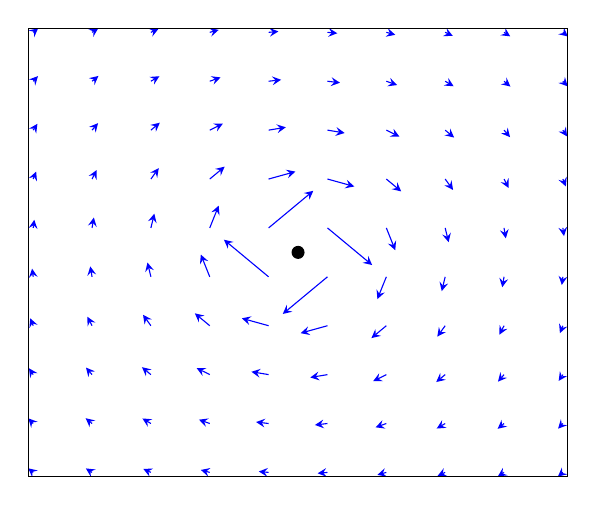
\begin{tikzpicture}
	\begin{axis}[domain=-2:2, view={0}{90}]
	\addplot3[blue, quiver={u={y/(x^2+y^2)}, v={-x/(x^2+y^2)}, scale arrows=0.15}, -stealth,samples=10] {0};
	\draw(0,0)node[circle, fill=black,scale=0.5]{};   
	\end{axis}          
\end{tikzpicture}
\end{document}
